%!TEX root = ../PatilM-[RnD-MT]Report.tex

\chapter{State of the Art}
\paragraph{}Over the years, research into qualitative spatial representations has led to the development of various models which can be used to represent the visually observable space.From a more scientific perspective these models are known as ``Qualitative calculi'', the current state of the art calculi rely on a single spatial primitive such as distance, direction, topology etc., to describe a set of relationships amongst the observable objects. In general each calculi comes with its own set of benefits and drawbacks as each one of them has been tailored to exploit different aspects of space\cite{bibid}. 

\paragraph{}For the case of robot navigation, current state of the art approaches utilize qualitative calculi that can provide both spatial and temporal information such as the QTC \cite{bibid} or QRPC \cite{bibid}. There exist comprehensive surveys that provide detailed information about each of the existing qualitative calculi\cite{bibid}, hence this state of the art aims to provide only a concise overview of the qualitative calculi that are advantageous to our application. We shall look into the relationships afforded by each of these calculi and their classification based on the domain of their utility.
 
\section{Forms of qualitative spatial representations}
		%    \item \textcolor{blue}{What have other people done?}
		%    \item The work presented in Alan Blackwell's master thesis \cite{blackwell1988spatial} provides a qualitative method for  representation of two dimensional shape and position and has been used to solve a few simple spatial reasoning tasks, with applications in the field of robotics. While the focus is mainly on the development of a qualitative representation it doesn't particularly focus on the use of this method for robot navigation. The outlined approaches for the use case in robot navigation raises more questions instead of providing a solid practical approach to the problem. 
		
		
		%    \item \cite{chao2014survey}
		%	\item \cite{dondrup2015computational}
		
		\subsection{Topological Representations} \cite{} \cite{bibid} \cite{bibid} : This is the most fundamental spatial representation, wherein the observed space is divided into distinctive regions based either on distinctive points in space or on separable objects found in the space. Topological representations draw heavily from the field of ``Mereology''(the theory of parthood) to describe relations between the distinctive regions. Qualitative calculi such as RCC, Interval Algebra, n-intersections etc. belong to this category. Such representations deal with the ``\textit{invariant properties that are under continuous deformations of objects, including translating, rotating and scaling}'', and often include only spatial information while completely disregarding temporal data. 
		
		\begin{figure}[h]
			\centering
			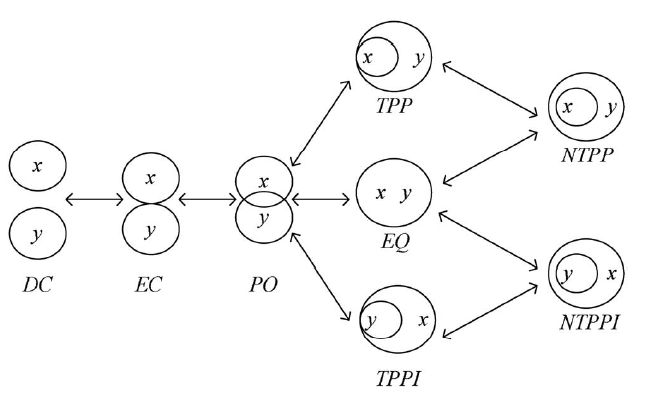
\includegraphics[width=0.7\linewidth]{images/rcc8_rel}
			\caption{The eight jointly exhaustive and pairwise disjoint relations of region connection calculus (RCC8). The arrows show which relation is the next relation a configuration would transit to, assuming the continuous movements or deformations \cite{bibid}, \cite{bibid}, \cite{bibid}.}
			\label{fig:rcc8rel}
		\end{figure}
		
		
		\subsection{Directional Representations} \cite{chen2015survey} : The relative direction between two different objects can be represented using directional relations/representations. These representations rely on three primary elements, a reference object, a reference frame and a target object to define a valid relation between two different objects. Directional representations are widely classified into two categories, point based and projection based with the discerning factor being the dimension of the objects involved and distinction of space using either cone shaped spatial sectors or by using vertical and horizontal lines to create smaller rectangular sectors. Furthermore, the directional calculus isn't restricted to using only cardinal directions, it also allows the use of nominal directional information such as left ,right etc to describe the directional relations. Qualitative calculi such as CDC, OPRA, CyCord etc utilize the directional representation. Being based of topological representations, directional representations also include only spatial information while disregarding temporal data.
		
		\begin{figure}[h!]%
			\centering
			\subfloat[Cone-shaped direction relations \cite{isli1}]{{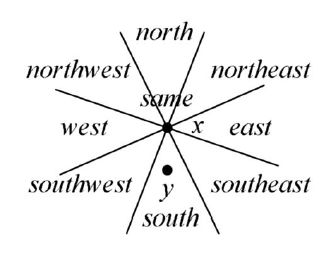
\includegraphics[width=6cm]{images/direction_cone} }}%
			\qquad
			\subfloat[Projection-based direction relations \cite{isli2}]{{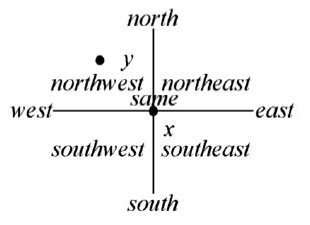
\includegraphics[width=6cm]{images/direction_projection} }}%
			\caption{The point based and projection based direction representations \cite{bibid}}%
			\label{fig:example}%
		\end{figure}
	
		\subsection{Distance Representations} \cite{chen2015survey} : The qualitative representation of spatial distance can be classified into two groups namely absolute and relative. This classification is made solely on the basis of  the presence/absence of an extraneous referential object in the relation between two objects. This distinction can be clearly illustrated by the following example,`the distance between A and B is 8 meters' or `A is near B', this is a absolute approach as the distance is measured directly between two objects.Whereas saying that `A is closer to B than that to C' classifies as a relative approaches as this involves the comparison to a third object.Furthermore, it has been shown that absolute approaches	can be qualitative or quantitative, but relative approaches are commonly qualitative \cite{bibid}.Qualitative calculi such as the ARGD(or Delta) and TPCC use the distance representations to describe the observable space. Distance based relations have found to be insufficient by themselves when it comes to the task of robot manipulation/navigation and hence are often used in combination with distance representations to yield a fairly suitable and complete representation of the environment \cite{bibid}. Like with the direction representations this calculi also lacks temporal data in the encoded relations and is hence unsuitable for applications involving moving objects.
		
		\begin{figure}[h]
			\centering
			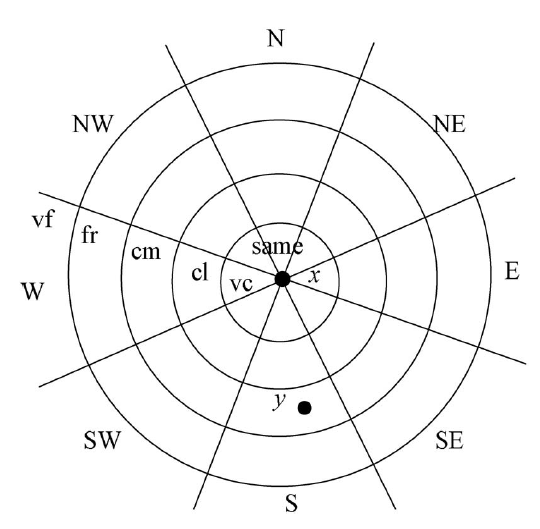
\includegraphics[scale=0.8]{images/argd_delta}
			\caption{An representation of the combination of cone-shaped direction and absolute distance: very
				close(vc), close(cl), commensurate(cm), far(fr) and very far(vf), \cite{clementini1997qualitative}.}
			\label{fig:argddelta}
		\end{figure}
		
		
		\subsection{Moving object Representations} \cite{chen2015survey} : Topological representations, directional representations and distance representations describe relations between stationary objects, this limitation encouraged the development of a moving object representation which can qualitatively represent moving objects and their trajectories. These representations effectively deal with both spatial and temporal data to describe valid relations among mobile objects, while these relations include some directional information they mainly describe the relative motion between two objects and not relative direction. The relative motion between two objects is described using oriented line segments which are approximations of the trajectory of the objects in motion. QTC, QRPC are the two prominent calculi that utilize moving object representations. Moving object representations and the calculi using these representations have been proven to have solved the problem of representing moving objects but since these relations lack any distance information, they are still prone to failure and often need a complimentary distance calculi to ensure that a mobile object(robot) can successfully move around in the given environment without collisions.
		
		\begin{figure}[h]
			\centering
			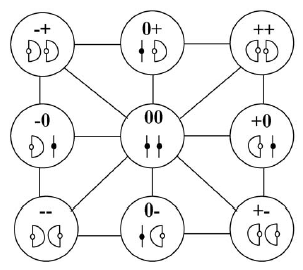
\includegraphics[scale=1]{images/qtcb}
			\caption{Basic relations of basic Qualitative Trajectory Calculus (QTCB) in a conceptual neighborhood diagram. The solid dots represent the stationary objects and the open dots represent the moving objects \cite{bibid}, \cite{de_weghe}.}
			\label{fig:qtcb}
		\end{figure}		
		
		\newpage
		
		\begin{table}[h!]
			\begin{adjustwidth}{-2cm}{}
				\resizebox{\textwidth}{!}{%
					\begin{tabular}{|p{3cm}|p{4cm}|p{3cm}|p{3cm}|p{8cm}|}
						\hline
						\textbf{Domain} & \textbf{Model Name} & \textbf{Type of objects} &\textbf{Number and granularity of relationships} & \textbf{Description} \\ \hline
						\multirow{2}{*}{Temporal} & Interval Algebra \cite{allen1990maintaining} & Time Intervals & 13 relationships, Binary relationships & It does not consider time instants. \\ \cline{2-5} 
						& Extended Interval Algebra  \cite{freksa1992temporal} & Time intervals and extreme points of the intervals & 29 (13 IA(Interval algebra) + 16 extremes), binary & It extends IA(Interval Algebra) model by considering new relationships including the extremes of the interval and it introduces the notion of conceptual neighborhood. \\ \hline
						\multirow{8}{*}{Spatial} & Region Connection Calculus  \cite{randell1992spatial} & Sets & 8 or 5 relationships, Binary Relationships & It uses the geometric properties associated to the connection between two sets to establish relationships that are no longer linear but planar, and which are invariant to translation, rotation and scaling. \\ \cline{2-5} 
						& Cardinal Reference System(CRS)  \cite{frank1992qualitative} & Generic objects & 9 (8 cardinals + 1 neutral) relations, Binary Relationships & It describes the position of any object by using a cardinal orientation as reference system and by adding also a neutral region \\ \cline{2-5} 
						& FFC (Flip Flop Calculus) \cite{ligozat1998reasoning} & Points & 8 (6 + 1 double + 1 triple), Ternary Relations & It is based on the possible positions of a point C with respect to a segment AB defined by other two points, A and B. \\ \cline{2-5} 
						& SCC (Single Cross Calculus) \cite{freksa1992temporal} & Points & 11 (8 +B=C+1 double + 1 triple), Ternary Relations & Describes the possible positions of a point C with respect to a segment AB and the orthogonal line to segment AB on B. \\ \cline{2-5} 
						& DCC (Double Cross Calculus)  \cite{freksa1992utilization} & Points & 17 (15 regions + 1 double + 1 triple), Ternary Relations & Describes the possible positions of a point C with respect to a segment AB and two orthogonal lines to segment AB on A and B. \\ \cline{2-5} 
						& Oriented point based Reasoning  \cite{moratz2006representing}& Oriented Points & 4, Binary Relations & It is based on the relative orientation between pairs of oriented points in terms of two qualitative spatial dichotomies: the front–back and left–right. \\ \cline{2-5} 
						& DRA (Dipole Relation Algebra)  \cite{dylla2004empirical}, \cite{dylla2004exploiting} & Dipoles (or oriented segments) & 24, Binary Relations & It is based on the relative position of oriented segments. \\ \cline{2-5} 
						& OPRA (Oriented Point Relation Algebra)  \cite{dylla2006generalizing} & Oriented points & Depends on the granularity, Binary Relations & As DRA model, it is also based on the relative position two oriented points, but it supports different levels of granularity. \\ \hline
						\multirow{2}{*}{Spatio-temporal} & QTC (Qualitative Trajectory Calculus)  \cite{van2005representing} & Points & 81, Binary Relations & It describes the possible relations among two moving points in terms of the front–back and left–right dichotomies. \\ \cline{2-5} 
						& QRPC (Qualitative Rectilinear Projection Calculus)  \cite{glez2013qrpc} & Oriented points & Depends on the chosen granularity (up to 48), Ternary Relations & It establishes the possible relations of an object with respect to the trajectory of another object depending on the cross-point of the trajectories and the relative position among them \\ \hline
				\end{tabular}}
			\caption{Key features of the more representative models(calculi) of qualitative representations of spatial or temporal domains in the existing literature \cite{glez2013qrpc}.}
			\end{adjustwidth}
		\end{table}
	
			\newpage
	
		\subsection{Conclusion:}From the above breakdown of the representations and the calculi, it is easy to summarize that distance representations and moving object representations are the most promising representations for our application in mobile robot navigation. Consequently the calculi associated with these representations will be the ones that are further scrutinized in the following section. The reasoning behind this conclusion is fairly simple moving object representations are basically spatio-temporal representations which take into account both the spatial and temporal data to create abstractions of the objects trajectory, this is crucial when dealing with mobile objects as this gives a more concrete representation of the objects in motion. In the case of distance representations although these representations deal only with spatial information, they provide explicit information on how close or far the objects under consideration are. Thus effectively capturing the possibility of a collision between the objects, this sort of information cannot be found in the direction and topological representations hence rendering them unfavorable for our application in mobile robot navigation \cite{chen2015survey}, \cite{cohn1997qualitative}, \cite{cohn2001qualitative}, \cite{cohn2008qualitative} and maybe \cite{Yan2012QualitativeRA}.
	
	\section{Analyzing qualitative calculi for navigation}
	\paragraph{} This section aims to provide a through understanding at a selective group of qualitative calculi based on the conclusions drawn from the previous section. Namely we shall look at the qualitative calculi such as the QTC, QRPC and ARGD which use moving object representations and distance representations and function in the spatio-temporal and spatial domains respectively.
%	write only theory here
	\subsection{Qualitative Trajectory calculus}
	\paragraph{\cite{van2004representing}, \cite{van2006qualitative}, \cite{van2005qualitative}}The QTC calculus was developed to solve the problem of inadequate representation of mobile objects in the spatio-temporal domain, which until then were represented only in the spatial domain using either the RCC or the n-intersections calculi. The major drawbacks of those calculi was their failure to deal with temporal data. Hence mobile objects were often abstracted as stationary regions using either 'disconnected from' relation (DC) in RCC or 'disjoint' relation in the 9-intersection model, with the exception of a few limiting cases where the two objects meet, such as a collision between two mobile robots.Thus, the limiting factor of these formalisms was that all the DC relations were non-differentiable, due to the ignorance of information regarding relative motion between the two objects.
	\paragraph{}The QTC calculus constitutes of two major variants the $QTC_B$ and the $QTC_C$, with the major difference between the two being the inclusion of the directional information in the relationships(between two objects) of the $QTC_C$ calculus. Both versions of the QTC are adept at dealing with qualitative movement of objects in one, two and three dimensions. In the $QTC_B$ calculus, as the euclidean distance between two objects is taken as the only constraining dimension.The abstraction of movement is depicted using three qualitative values:
	\begin{itemize}
		\item 0: the object is stable with respect to the other object.
		\item -: the object is moving towards the other object.
		\item +: the object is moving away from the other object.
	\end{itemize}
	The assigning of these qualitative values to an object's movement depends upon the relative position(constrained by distance) and relative speed of the two objects with respect to each other. This can be illustrated by the following example, consider two objects `j' and `k', the possible values for `j' :
	
	\begin{itemize}
		\item based on relative position at a time `t' are:
		\begin{enumerate}
			\item 0 (stable): if there is no change in the relative position with respect to `k' (no change in relative distance ).
			
			\item - (moving towards): if there is a change in the relative position with respect to `k', such that the relative distance between the objects decreases.
			
			\item + (moving away): if there is a change in the relative position with respect to `k', such that the relative distance between the objects increases.
		\end{enumerate}
		\item based on relative speed at a time `t' are:
		\begin{enumerate}
			\item 0 (stable): if speed of `j' is equal to the speed of `k'.
			
			\item - (moving towards): if speed of `j' is lesser than the speed of `k'.
			
			\item + (moving away): if speed of `j' is greater than the speed of `k'.
		\end{enumerate}
	\end{itemize}

	\paragraph{}Hence a valid $QTC_B$ relation between qualitative trajectories of two objects is represented as such `{-,+,-}'(for object 1) and `{+,-,+}' (for object two). Wherein the value in the first position is the relative position of the object in consideration, the second value is the relative position of the other object and the third value is the relative speed of the current object with respect to the other object. The benefit of having a relation that includes both relative position and speed comes to light when dealing with the movement of objects in higher dimensions(2D, 3D) for instance in 2D, the value `0'(stable) may be interpreted as either the distance being stable or the speed being stable, this confusion during interpretation is avoided by using unique values for both the relative distance and speed and hence the size of the resulting relations is a set of three. Interpretation of these relations is pretty straight-forward when dealing with movements one dimension.
	
	\paragraph{}The $QTC_C$ variation of the QTC calculus is often seen as an extension of the $QTC_B$ calculus, since it uses the same qualitative values to represent the qualitative trajectories of the objects. The only difference between the two versions comes from the integration of directional information which denotes the direction of movement of the current object in relation to a line segment between the two objects. This version of the QTC calculus was inspired in part by the `Double cross calculus' \cite{zimmermann1996qualitative}, hence the name. The $QTC_C$ calculus is an improvement on the double cross calculus, as it can define qualitative trajectories and direction for single as well as multiple objects at once, whereas the double cross calculus can only deal with single objects at any given instance of time.
	
	\newpage
	
	\begin{figure}[h!]
		\centering
		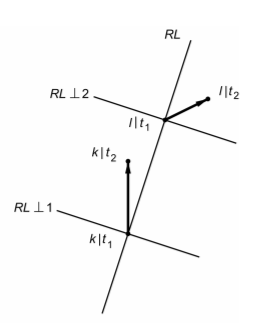
\includegraphics[scale=1]{images/QTCC}
		\caption{A graphical representation of the $QTC_C$ calculus for a relation between two moving objects`k' and `l', where $t_1$ and $t_2$ are the two distinctive time instances and RL refers to the reference line and the double crosses($RL\perp1$, $RL\perp2$) for the two objects \cite{van2005qualitative} .}
		\label{fig:qtcc}
	\end{figure}

	\paragraph{}The relations of the $QTC_C$ calculus, while following the same basic principles of the $QTC_B$, have been tweaked slightly to allow inferencing of the objects position in terms of the relative direction to the reference line. The assignment of the qualitative values to the object's movements can be illustrated using two objects `k' and `l', the possible values for `l' at any given time interval are based on the following reasoning:
	
	\begin{itemize}
		\item based on movement relative to the respective perpendicular reference line:
		
		\begin{enumerate}
			\item 0 (stable): if there is no change in the relative distance with respect to `k' or with respect to the reference line. 
			
			\item - (moving towards): if there is an increase in the relative distance between the objects.
			
			\item + (moving away): if there is an increase in the relative distance between the objects.
		\end{enumerate}
	
		\item  based on movement relative to the directed perpendicular reference line(from `l' to `k'):
		
		\begin{enumerate}
			\item 0 (moving along the directed reference line): if the object moves
			along the line segment or if it was moving along the left/right and continues to do so in the given time interval.
			
			\item - (moving to left side of the directed reference line): if the object moves from the right side of the line segment to the left side in the given time interval.
			
			\item + (moving to right side of the directed reference line): if the object moves from the left side of the line segment to the right side in the given time interval.
		\end{enumerate}
	
	\end{itemize}

	\paragraph{}Hence a valid $QTC_C$ relation between qualitative trajectories of two objects is represented as such `{-,+,-,0}'(for object 1) and `{+,-,-,0}'(for object two). Wherein the value in the first position is the relative position of the object in consideration, the second value is the relative direction of its movement, the third value is the relative position of the other object and the fourth is it's relative direction of movement.
	
	\paragraph{Conclusion}\cite{van2004representing}In conclusion it is safe to say that the $QTC_B$, calculi is more complete and robust in the sense that it can qualitatively and correctly represent all possible trajectories of the mobile object at a given instance of time, although due to it being developed to deal with mobile objects when they are in DC regions \cite{van2006qualitative} it still cannot make a very robust or accurate relation regarding collision conditions, it provides a safer alternative to the $QTC_C$ calculus as this calculus is still regarded as a work in progress \cite{van2005qualitative}due to it's inability to distinguish between the trajectories of a mobile object moving along the directed reference line and continuing to do so and a mobile object moving on either side of the directed reference line and continuing to do so. Thus this justifies the selection of $QTC_B$ for our implementation, not only is it safer and simpler but it also allows easier integration with other complimentary calculi such as ARGD, RCC which may be used to deal with possible collision cases.

	\subsection{Qualitative Rectilinear Projection calculus}
	\paragraph{\cite{glez2013qrpc}, \cite{alvarez2006guide}} The qualitative rectilinear projection calculus(QRPC) presents a innovative approach to qualitatively representing motion patterns based on planar trajectories. In comparison to the QTC calculus, this representation has a richer description of the motion exhibited by mobile objects. The basis of this claim lies in the oriented rectilinear projection used to represent the trajectories, which allows this calculus to represent rotational motions of an mobile object, something that was not possible in the existing calculi such as the QTC. The QRPC is specifically tailored towards obstacle avoidance and geometric relationships between two objects are generated using the front-back and the left-right dichotomies. The relationships encompassed in the QRPC abstract the objects as points and use their rectilinear projections to make qualitative distinctions such as front-back and left-right, these atomic relations and their base notations are illustrated below:
	
	\begin{enumerate}
		\item \textbf{Notations:}
		
		\begin{itemize}
			\item $P_iP_j$: is the relative disposition between the oriented rectilinear	projection of the object $O_i$ and the oriented rectilinear projection of $O_j$.
			\item $O_iO_j^{LR}$: The relative position of $O_i$ with respect to the left-right dichotomy of $O_j$.
			\item $({CO_i}^{FB})({CO_j}^{FB})$: The relative position of the point of intersection(`C') of the oriented rectilinear projections with respect to the front–back dichotomy of both objects.
			\item $O_iO_j^{FB}$:  The relative position of $O_i$ with respect to the front-back dichotomy of $O_j$ when the trajectories are superimposed.
			
			Note: `i' and `j' denote the two different objects.
		\end{itemize}
		
		\item \textbf{Qualitative (atomic)relations in each of the notations :}
		\begin{itemize}
			\item The relative disposition between two oriented rectilinear projections($P_iP_j$):
			
			\begin{itemize}
				\item  $\uparrow \uparrow$  : Parellel in same direction
				\item $\uparrow \downarrow$  : Parellel in opposite direction
				\item $\uparrow$  : Coincident in same direction
				\item $\updownarrow$  : Coincident in opposite direction 
				\item $X$  : Crossed/Intersecting rectilinear projections 
			\end{itemize}
		
			\item The relative position of $O_i$ with respect to the left-right
			dichotomy of $O_j$, ($O_iO_j^{LR}$):
			\begin{itemize}
				\item `-' : if $O_i$ is on the left of $P_j$.
				\item `0' : if $O_i$ is over $P_j$.
				\item `+' : if $O_i$ is on the right of $P_j$.
				
				\begin{figure}[h]
					\centering
					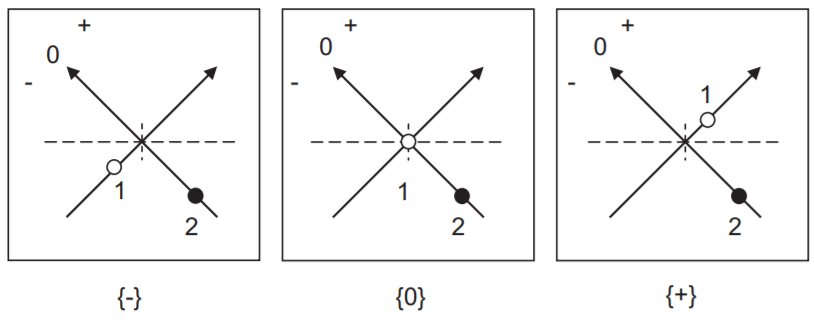
\includegraphics[width=0.7\linewidth]{images/QRPC_FB}
					\caption{Relative position of $O_i$ w.r.t the left-right dichotomy of $O_j$ for crossed projections \cite{glez2013qrpc}.}
					\label{fig:qrpcfb}
				\end{figure}
				
			\end{itemize}
			
			\item The relative position of `C' with respect to the front-back
			dichotomy of two objects $(CO_i^{FB})(CO_j^{FB})$:
			\begin{itemize}
				\item $(+,+)$ : if `C' is in front of $O_i$ and $O_j$.
				\item $(0,+)$ : if `C' is at same position as $O_i$ and in front of  $O_j$.
				\item $(+,-)$ : if `C' is in front of $O_i$ and behind $O_j$.
				\item $(0,-)$ : if `C' is at same position as $O_i$ and behind $O_j$.
				\item $(-,+)$ : if `C' is behind $O_i$ and in front of $O_j$.
				\item $(-,0)$ : if `C' is behind $O_i$ and in same position as $O_j$.
				\item $(-,-)$ : if `C' is behind $O_i$ and $O_j$.
				\item $(+,0)$ : if `C' is in front of $O_i$ and at the same position as $O_j$.
				\paragraph{}In cases where the two projections do not intersect with each other($\uparrow \uparrow$ or $\uparrow \downarrow$), this qualitative abstraction presents as conundrum as the point of intersection `C' may lie at either positive or negative infinity, hence in such cases the relation is abstracted to either $(+,+)$ or $(-,-)$.
				
				\begin{figure}[h]
					\centering
					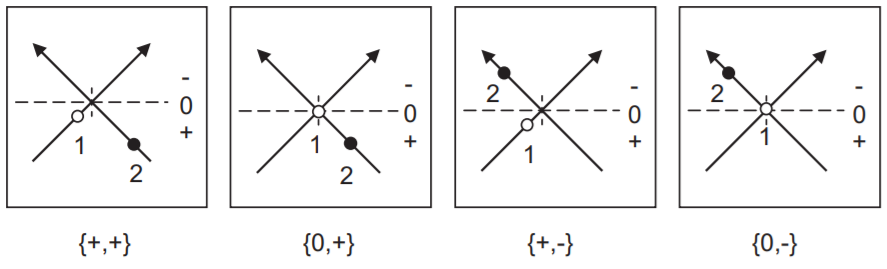
\includegraphics[width=0.7\linewidth]{images/QRPC_PJ}
					\caption{Some of the spatial configurations of the intersection point with respect to the front-back dichotomy of two objects for crossed projections $(CO_i^{FB})(CO_j^{FB})$, \cite{glez2013qrpc}.}
					\label{fig:qrpcpj}
				\end{figure}
				
			\end{itemize}
		\item The relative position of $O_i$ with respect to the front-back dichotomy of $O_j$ when the trajectories are superimposed($O_iO_j^{FB}$):
		\begin{itemize}
			\item `+' : if $O_i$ is in front of $O_j$ after $P_i$ is superimposed on $P_j$.
			\item `0' : if $O_i$ is at the same position as $O_j$ after $P_i$ is superimposed on $P_j$.
			\item `-' : if $O_i$ is behind $O_j$ after $P_i$ is superimposed on $P_j$.	
			
			
			Note: The after the rectilinear projection of $O_i$ is rotated(such that the objects are always facing in opposing directions) along `C' if it exists, before being superimposed on the rectilinear projection of $O_j$.		
		
			\begin{figure}[h!]%
				\centering
				\subfloat[The ($O_iO_j^{FB}$) feature for crossed projections. \cite{glez2013qrpc}]{{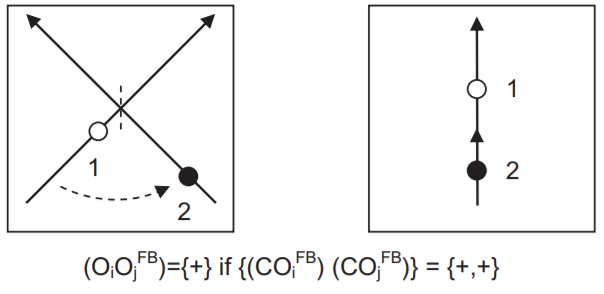
\includegraphics[width=6cm]{images/QRPC_ob1} }}%
				\qquad
				\subfloat[The ($O_iO_j^{FB}$) feature for parellel projections. \cite{glez2013qrpc}]{{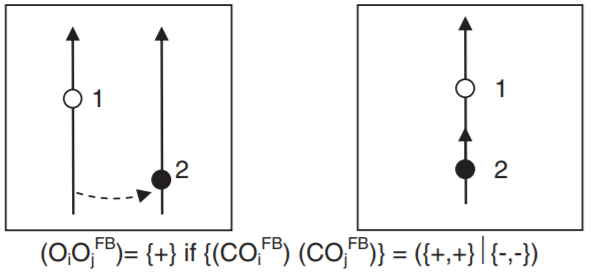
\includegraphics[width=6cm]{images/QRPCob2} }}%
				\caption{The point based and projection based direction representations \cite{bibid}}%
				\label{fig:QRPC superimposed}%
			\end{figure}
			
		\end{itemize}
	
		\end{itemize}
	\end{enumerate}
	\paragraph{Conslusion}Hence a complete valid QRPC relation comprising of the above mentioned atomic relations can be written as [($P_iP_j$)($O_iO_j^{LR}$)($({CO_i}^{FB})({CO_j}^{FB})$)($O_iO_j^{FB}$)], with the various values replacing their respective placeholders. Thus proving to be a richer representation of the movements of the mobile objects as it can effectively distinguish  between front-back, left-right as well as same or opposing direction of heading. While this calculus does present a compact view of the movements of the objects, like it's predecessors it still requires a sequence of qualitative(QRPC) states(individual sets of relations) to effectively represent the movement of an object, besides a completely theoretical formulation of the calculi without the backing of suitable empirical data or implementation makes it hard to believe that this calculi would function reliably in a real time mobile robot scenario. These drawbacks dissuade us from further pursuing this calculi for our purpose of achieving qualitative perception and control in mobile robots. 
	
	\subsection{Qualitative Distance calculus}
	\paragraph{\cite{clementini1997qualitative}}
	

	\section{Implementations of qualitative calculi for navigation}
	
	\begin{itemize}
	\item \cite{chen2006qualitative}, utilizes a teach-relay approach to navigate through indoor and outdoor environments. A sparse optical flow technique is used to extract features in the teach phase and feature matching is done in the replay phase to successfully navigate a given path. The approach uses a qualitative control strategy where motion primitives are obtained by using a voting mechanism in collaboration with the observed features.
	\item \cite{chen2009qualitative},develops a qualitative control algorithm that is able to navigate through both indoor and outdoor environments by using a concept called funnel lane, where the feature coordinates are used to determine turning directions in the replay phase. The algorithm couples odometry information with the funnel lane approach to achieve robust navigation.
	
	\subsection{Implementations}{Examples of implementation of navigation using qualitative control}
	\item \cite{sarcinelli2002using} The research presented in this approach uses optical flow vectors in combination with a confidence measure to control the linear and angular speeds of the robot. Image segmentation is used to split the scene into different objects and a estimation of time of collision for each object is used as a confidence measure for the control commands.
	\item \cite{murali2008autonomous} This approach uses a single monocular gray-scale camera to navigate. The algorithm uses a combination of visual homing and corridor ceiling lights to perform straight-line navigation in an unknown corridor. Although this approach works with both textured and untextured environments it uses a kalman filter(quantitative approach) to achieve localization.

\end{itemize}m

\section{....}
Use as many sections as you need in your related work to group content into logical groups

\section{Limitations of previous work}

